% Options for packages loaded elsewhere
\PassOptionsToPackage{unicode}{hyperref}
\PassOptionsToPackage{hyphens}{url}
%
\documentclass[
]{book}
\usepackage{amsmath,amssymb}
\usepackage{lmodern}
\usepackage{ifxetex,ifluatex}
\ifnum 0\ifxetex 1\fi\ifluatex 1\fi=0 % if pdftex
  \usepackage[T1]{fontenc}
  \usepackage[utf8]{inputenc}
  \usepackage{textcomp} % provide euro and other symbols
\else % if luatex or xetex
  \usepackage{unicode-math}
  \defaultfontfeatures{Scale=MatchLowercase}
  \defaultfontfeatures[\rmfamily]{Ligatures=TeX,Scale=1}
\fi
% Use upquote if available, for straight quotes in verbatim environments
\IfFileExists{upquote.sty}{\usepackage{upquote}}{}
\IfFileExists{microtype.sty}{% use microtype if available
  \usepackage[]{microtype}
  \UseMicrotypeSet[protrusion]{basicmath} % disable protrusion for tt fonts
}{}
\makeatletter
\@ifundefined{KOMAClassName}{% if non-KOMA class
  \IfFileExists{parskip.sty}{%
    \usepackage{parskip}
  }{% else
    \setlength{\parindent}{0pt}
    \setlength{\parskip}{6pt plus 2pt minus 1pt}}
}{% if KOMA class
  \KOMAoptions{parskip=half}}
\makeatother
\usepackage{xcolor}
\IfFileExists{xurl.sty}{\usepackage{xurl}}{} % add URL line breaks if available
\IfFileExists{bookmark.sty}{\usepackage{bookmark}}{\usepackage{hyperref}}
\hypersetup{
  pdftitle={Statistics for Psychologists},
  pdfauthor={John Towse, Tom Beesley, Margriet Groen, Rob Davies},
  hidelinks,
  pdfcreator={LaTeX via pandoc}}
\urlstyle{same} % disable monospaced font for URLs
\usepackage{color}
\usepackage{fancyvrb}
\newcommand{\VerbBar}{|}
\newcommand{\VERB}{\Verb[commandchars=\\\{\}]}
\DefineVerbatimEnvironment{Highlighting}{Verbatim}{commandchars=\\\{\}}
% Add ',fontsize=\small' for more characters per line
\usepackage{framed}
\definecolor{shadecolor}{RGB}{248,248,248}
\newenvironment{Shaded}{\begin{snugshade}}{\end{snugshade}}
\newcommand{\AlertTok}[1]{\textcolor[rgb]{0.94,0.16,0.16}{#1}}
\newcommand{\AnnotationTok}[1]{\textcolor[rgb]{0.56,0.35,0.01}{\textbf{\textit{#1}}}}
\newcommand{\AttributeTok}[1]{\textcolor[rgb]{0.77,0.63,0.00}{#1}}
\newcommand{\BaseNTok}[1]{\textcolor[rgb]{0.00,0.00,0.81}{#1}}
\newcommand{\BuiltInTok}[1]{#1}
\newcommand{\CharTok}[1]{\textcolor[rgb]{0.31,0.60,0.02}{#1}}
\newcommand{\CommentTok}[1]{\textcolor[rgb]{0.56,0.35,0.01}{\textit{#1}}}
\newcommand{\CommentVarTok}[1]{\textcolor[rgb]{0.56,0.35,0.01}{\textbf{\textit{#1}}}}
\newcommand{\ConstantTok}[1]{\textcolor[rgb]{0.00,0.00,0.00}{#1}}
\newcommand{\ControlFlowTok}[1]{\textcolor[rgb]{0.13,0.29,0.53}{\textbf{#1}}}
\newcommand{\DataTypeTok}[1]{\textcolor[rgb]{0.13,0.29,0.53}{#1}}
\newcommand{\DecValTok}[1]{\textcolor[rgb]{0.00,0.00,0.81}{#1}}
\newcommand{\DocumentationTok}[1]{\textcolor[rgb]{0.56,0.35,0.01}{\textbf{\textit{#1}}}}
\newcommand{\ErrorTok}[1]{\textcolor[rgb]{0.64,0.00,0.00}{\textbf{#1}}}
\newcommand{\ExtensionTok}[1]{#1}
\newcommand{\FloatTok}[1]{\textcolor[rgb]{0.00,0.00,0.81}{#1}}
\newcommand{\FunctionTok}[1]{\textcolor[rgb]{0.00,0.00,0.00}{#1}}
\newcommand{\ImportTok}[1]{#1}
\newcommand{\InformationTok}[1]{\textcolor[rgb]{0.56,0.35,0.01}{\textbf{\textit{#1}}}}
\newcommand{\KeywordTok}[1]{\textcolor[rgb]{0.13,0.29,0.53}{\textbf{#1}}}
\newcommand{\NormalTok}[1]{#1}
\newcommand{\OperatorTok}[1]{\textcolor[rgb]{0.81,0.36,0.00}{\textbf{#1}}}
\newcommand{\OtherTok}[1]{\textcolor[rgb]{0.56,0.35,0.01}{#1}}
\newcommand{\PreprocessorTok}[1]{\textcolor[rgb]{0.56,0.35,0.01}{\textit{#1}}}
\newcommand{\RegionMarkerTok}[1]{#1}
\newcommand{\SpecialCharTok}[1]{\textcolor[rgb]{0.00,0.00,0.00}{#1}}
\newcommand{\SpecialStringTok}[1]{\textcolor[rgb]{0.31,0.60,0.02}{#1}}
\newcommand{\StringTok}[1]{\textcolor[rgb]{0.31,0.60,0.02}{#1}}
\newcommand{\VariableTok}[1]{\textcolor[rgb]{0.00,0.00,0.00}{#1}}
\newcommand{\VerbatimStringTok}[1]{\textcolor[rgb]{0.31,0.60,0.02}{#1}}
\newcommand{\WarningTok}[1]{\textcolor[rgb]{0.56,0.35,0.01}{\textbf{\textit{#1}}}}
\usepackage{longtable,booktabs,array}
\usepackage{calc} % for calculating minipage widths
% Correct order of tables after \paragraph or \subparagraph
\usepackage{etoolbox}
\makeatletter
\patchcmd\longtable{\par}{\if@noskipsec\mbox{}\fi\par}{}{}
\makeatother
% Allow footnotes in longtable head/foot
\IfFileExists{footnotehyper.sty}{\usepackage{footnotehyper}}{\usepackage{footnote}}
\makesavenoteenv{longtable}
\usepackage{graphicx}
\makeatletter
\def\maxwidth{\ifdim\Gin@nat@width>\linewidth\linewidth\else\Gin@nat@width\fi}
\def\maxheight{\ifdim\Gin@nat@height>\textheight\textheight\else\Gin@nat@height\fi}
\makeatother
% Scale images if necessary, so that they will not overflow the page
% margins by default, and it is still possible to overwrite the defaults
% using explicit options in \includegraphics[width, height, ...]{}
\setkeys{Gin}{width=\maxwidth,height=\maxheight,keepaspectratio}
% Set default figure placement to htbp
\makeatletter
\def\fps@figure{htbp}
\makeatother
\setlength{\emergencystretch}{3em} % prevent overfull lines
\providecommand{\tightlist}{%
  \setlength{\itemsep}{0pt}\setlength{\parskip}{0pt}}
\setcounter{secnumdepth}{5}
\usepackage{booktabs}
\ifluatex
  \usepackage{selnolig}  % disable illegal ligatures
\fi
\usepackage[]{natbib}
\bibliographystyle{apalike}

\title{Statistics for Psychologists}
\author{John Towse, Tom Beesley, Margriet Groen, Rob Davies}
\date{2021-11-18}

\begin{document}
\maketitle

{
\setcounter{tocdepth}{1}
\tableofcontents
}
\hypertarget{intro}{%
\chapter{Intro}\label{intro}}

This is a collection of tuition material written for Psychology undergraduates at Lancaster University. At the moment the content represents the ``lab materials'' for the PSYC121 and PSYC122 modules in first year. They feature tuition of programming with R, with material designed to be accessible for students without any programming background.

\hypertarget{analysis-labs-and-pre-lab-work}{%
\section{Analysis labs and `pre-lab work'}\label{analysis-labs-and-pre-lab-work}}

Where the 121 Analysis lab includes a ``pre-lab'' section -- such as this one! -- please ensure you have (a) watched the relevant pre-recorded lecture material (b) read through \emph{this section} before your assigned lab class session and (c) completed any specified exercises.

The lecture is designed to deliver important ideas and procedures for learning about analysis. Pre-lab material is then designed to help consolidate this learning, or enhance, expand and apply it in ways that set the scene for the lab session activity. We want to prepare you to be ready to go in the session itself and make the most of your time there.

\begin{quote}
Top tip for part 1: Going into sessions prepared will help you get more out of the teaching.`

Getting an overview or briefing on what you will be doing by reading relevant material etc, means you know what to expect, and where to focus your energy. Don't be shy about coming with questions!
\end{quote}

\hypertarget{computing-systems}{%
\section{Computing systems}\label{computing-systems}}

For all University systems you will need to be a registered user and have received a `username` and details about how to generate your `password`. If you are struggling to set this up, then contact \href{https://www.lancaster.ac.uk/iss/help-and-support/}{ISS ASAP}.

All staff and students have e-mail accounts on the University system. Normally an e-mail address takes the form: first \href{mailto:initial.surname@lancaster.ac.uk}{\nolinkurl{initial.surname@lancaster.ac.uk}}

For example, to contact the Content Director of PSYC121, Tom Beesley, you use \href{mailto:t.beesley@lancaster.ac.uk}{\nolinkurl{t.beesley@lancaster.ac.uk}} (usually you can also use the shortened version, \href{mailto:t.beesley@lancs.ac.uk}{\nolinkurl{t.beesley@lancs.ac.uk}})

When the department needs to contact you individually we send a message to your \textbf{university e-mail account}. In addition, the University e-mail security system, specifically the SPAM prevention procedures, will frequently ``junk'' e-mail from external accounts from free systems (e.g., hotmail, google, etc.). It's always preferable to use your University email account so staff know it is a genuine student request.

Consequently we stress that you:

\begin{itemize}
\item
  DO NOT use external accounts when contacting the Department or Staff as messages from these are not guaranteed to be delivered (and are routinely not replied to by Staff)
\item
  Check your university account \underline{daily}, as important University and Departmental messages may be in this mailbox
\end{itemize}

\textbf{\emph{Moodle}}

Moodle plays a key role in your time at Lancaster. Moodle is the University VLE (Virtual Learning Environment). Moodle is used to:

\begin{itemize}
\item
  Communicate course information and urgent messages to all students on a course. As a result \textbf{it is essential for all students to log in at least once a day}
\item
  Make course materials, such as lectures, lecture slides/notes, and lab handouts, accessible to students prior to these sessions
\item
  Provide the web links for each Web-Based Assessment (WBA)
\item
  Provide forums for online discussions regarding course material (students are encouraged to use these forums to raise questions about course material that they seek clarity on)
\end{itemize}

\hypertarget{other-department-research-systems}{%
\section{Other Department research systems}\label{other-department-research-systems}}

\textbf{\emph{The Department SONA system}}

In your full online Part I handbook you can read about the Research Participation Scheme (run through the SONA system). This scheme offers students the opportunity to take part in research studies. The studies cover a range of research topics and are interesting to take part in. They provide an invaluable learning opportunity for students in terms of how to design experiments, how to treat participants in an ethical manner and how to run an experiment. Many research studies in the first term will be carried out by final-year undergraduates collecting data for their research projects. This may well be you in a couple of years time!

~Psychology students registered on PSYC121 are strongly encouraged to take part in these studies and collect a minimum of 20 credits* {[}* this is an estimate at the time of writing - the target will be communicated when confirmed within the department{]}. There are multiple incentives.

First, completion of these credits is an essential pre-requisite to use the SONA system to recruit participants to your own study when you enter your third year. (nb you are required to carry out your own research project as part of your Psychology degree). This benefit of this access should NOT be underestimated.

Second, once you have collected 20 credits, you will be able to collect additional credits, and earn further project credits for yourself in the third year. But also, taking part in studies, run by other undergraduates, or postgraduates or Research Assistants or staff, is a fantastic way to learn about research methods and experimental designs and psychology in general. Time and again, many students tell us that they got great ideas for projects and for good experiments from their experiences as participants. Being a research participant provides unique insights into what goes on in experiments and what we can learn from them.

You will receive more information about SONA -- such as how to register to gain access to studies -- in the next couple of weeks.

\hypertarget{week-1-introduction-to-statistics-with-r-studio}{%
\chapter{Week 1: Introduction to Statistics with R Studio}\label{week-1-introduction-to-statistics-with-r-studio}}

\begin{quote}
Written by John Towse \& Tom Beesley
\end{quote}

The exercises in this section are designed to familiarise you with working in R Studio.

\hypertarget{lab-work}{%
\section{Lab Work}\label{lab-work}}

\hypertarget{introducing-r-studio}{%
\subsection{Introducing R Studio}\label{introducing-r-studio}}

R and R Studio is the software that we will be using to explore and learn about analysis in your Psychology degree. It's a computational engine: a very snazzy calculator that you should see as your friend and ally in the journey to understand and appreciate psychology. It sits \emph{alongside} what we teach about the concepts and interpretation of statistical analysis.

R is the core software, R Studio is the interface for interacting with it. Put another way, \emph{R is the engine, R Studio is the cockpit.}

Like even a simplest calculator, it just does what you ask (at least when you ask nicely!) but it requires the user to know what they want from it and to understand what it is telling you. A calculator can't help a kid get the right answer to a multiplication problem if they don't know the difference between multiplication and division and addition etc. And whilst a calculator is brilliant at doing the number crunching (and as a bonus, R Studio can help with turning the numbers into beautiful graphs and images too), even a calculator requires a thoughtful person to take the answers and make sensible interpretations from them.

Therefore, we need to learn both about the concepts of statistical analysis on the one hand, and the processing of statistical information -through R- on the other. The lectures will provide the starting point and the direction for statistical concepts, whilst these analysis labs provide the more practical experiences in how to use R, and how to R your ally. Over the next year, in these labs we will increasingly be using R Studio to focus on the latter, processing side, which will allow you to focus your energies on the conceptual side and its relevance for appreciating psychology.

\hypertarget{getting_started}{%
\subsection{Getting started with R Studio}\label{getting_started}}

For Lancaster University Psychology Students in 2021, we will be learning about R Studio through a simple but powerful web server architecture. That is, through the power of the internet, you can access and use R Studio by logging into a free account that we have provided and we will maintain for your use.

\begin{quote}
Here's a little secret: There are several different ways to access R Studio. For example, you can download a copy of the software onto your computer, or use a Virtual Machine set up to run a copy. There's nothing to stop you having your local copy, but please note - we can't support your own version through lab classes
\end{quote}

So why are we using an R Studio web server?

\begin{itemize}
\item
  Uniformity of experience. It doesn't matter whether you have a PC, a Mac, a Chromebook or whatever. The server provides a consistent, uniform experience. That also means we can spend more time helping you master the software, rather than translating between versions on different platforms
\item
  Ubiquity of experience. There are \textbf{lots} of computers on campus. There are computer rooms, there are pods in the learning centre, there are bookable laptops in the Levy Lab, and so on. Providing a web interface from a browser, means you can practice R from all the different machines. Your not limited to a particular copy on a single machine.
\item
  Consistency of performance. Since everyone logs into the same installation of R Studio, we can ensure that things work the way we expect. This allows staff to focus on teaching you the key issues, without worrying about software conflicts because different machines have different configurations, or different versions with different features etc. We'll have more time to focus on the important stuff!
\item
  Quality of performance. Some installations of R Studio and some commercial versions of the server are set up, well, to be the basic version rather than the premium version. To draw a papelle: do you want to have to put up with the cheap, low-bandwidth broadband package? We've got control of the server set up, so we'll try and make this the most effective way to do this.
\end{itemize}

We've moved to the R Studio server approach this year. We've tried hard to set it up to work well- Apologies in advance for any teething issues, we will try to resolve them as quickly as possible.

You will have received an email with your account information to log onto the R Studio server. Please keep your account details safe.

From a computer on the campus wifi, you can access R Studio at:

\href{http://psy-rstudio.lancaster.ac.uk}{psy-rstudio.lancaster.ac.uk} (off campus, you will need to be on the VPN)

At the login screen, use your university username (e.g., bloggsj)

Your password for R Studio is: {[}password here{]}

\hypertarget{what-does-it-look-like}{%
\subsubsection{What does it look like?}\label{what-does-it-look-like}}

When RStudio starts, it will look something like this: 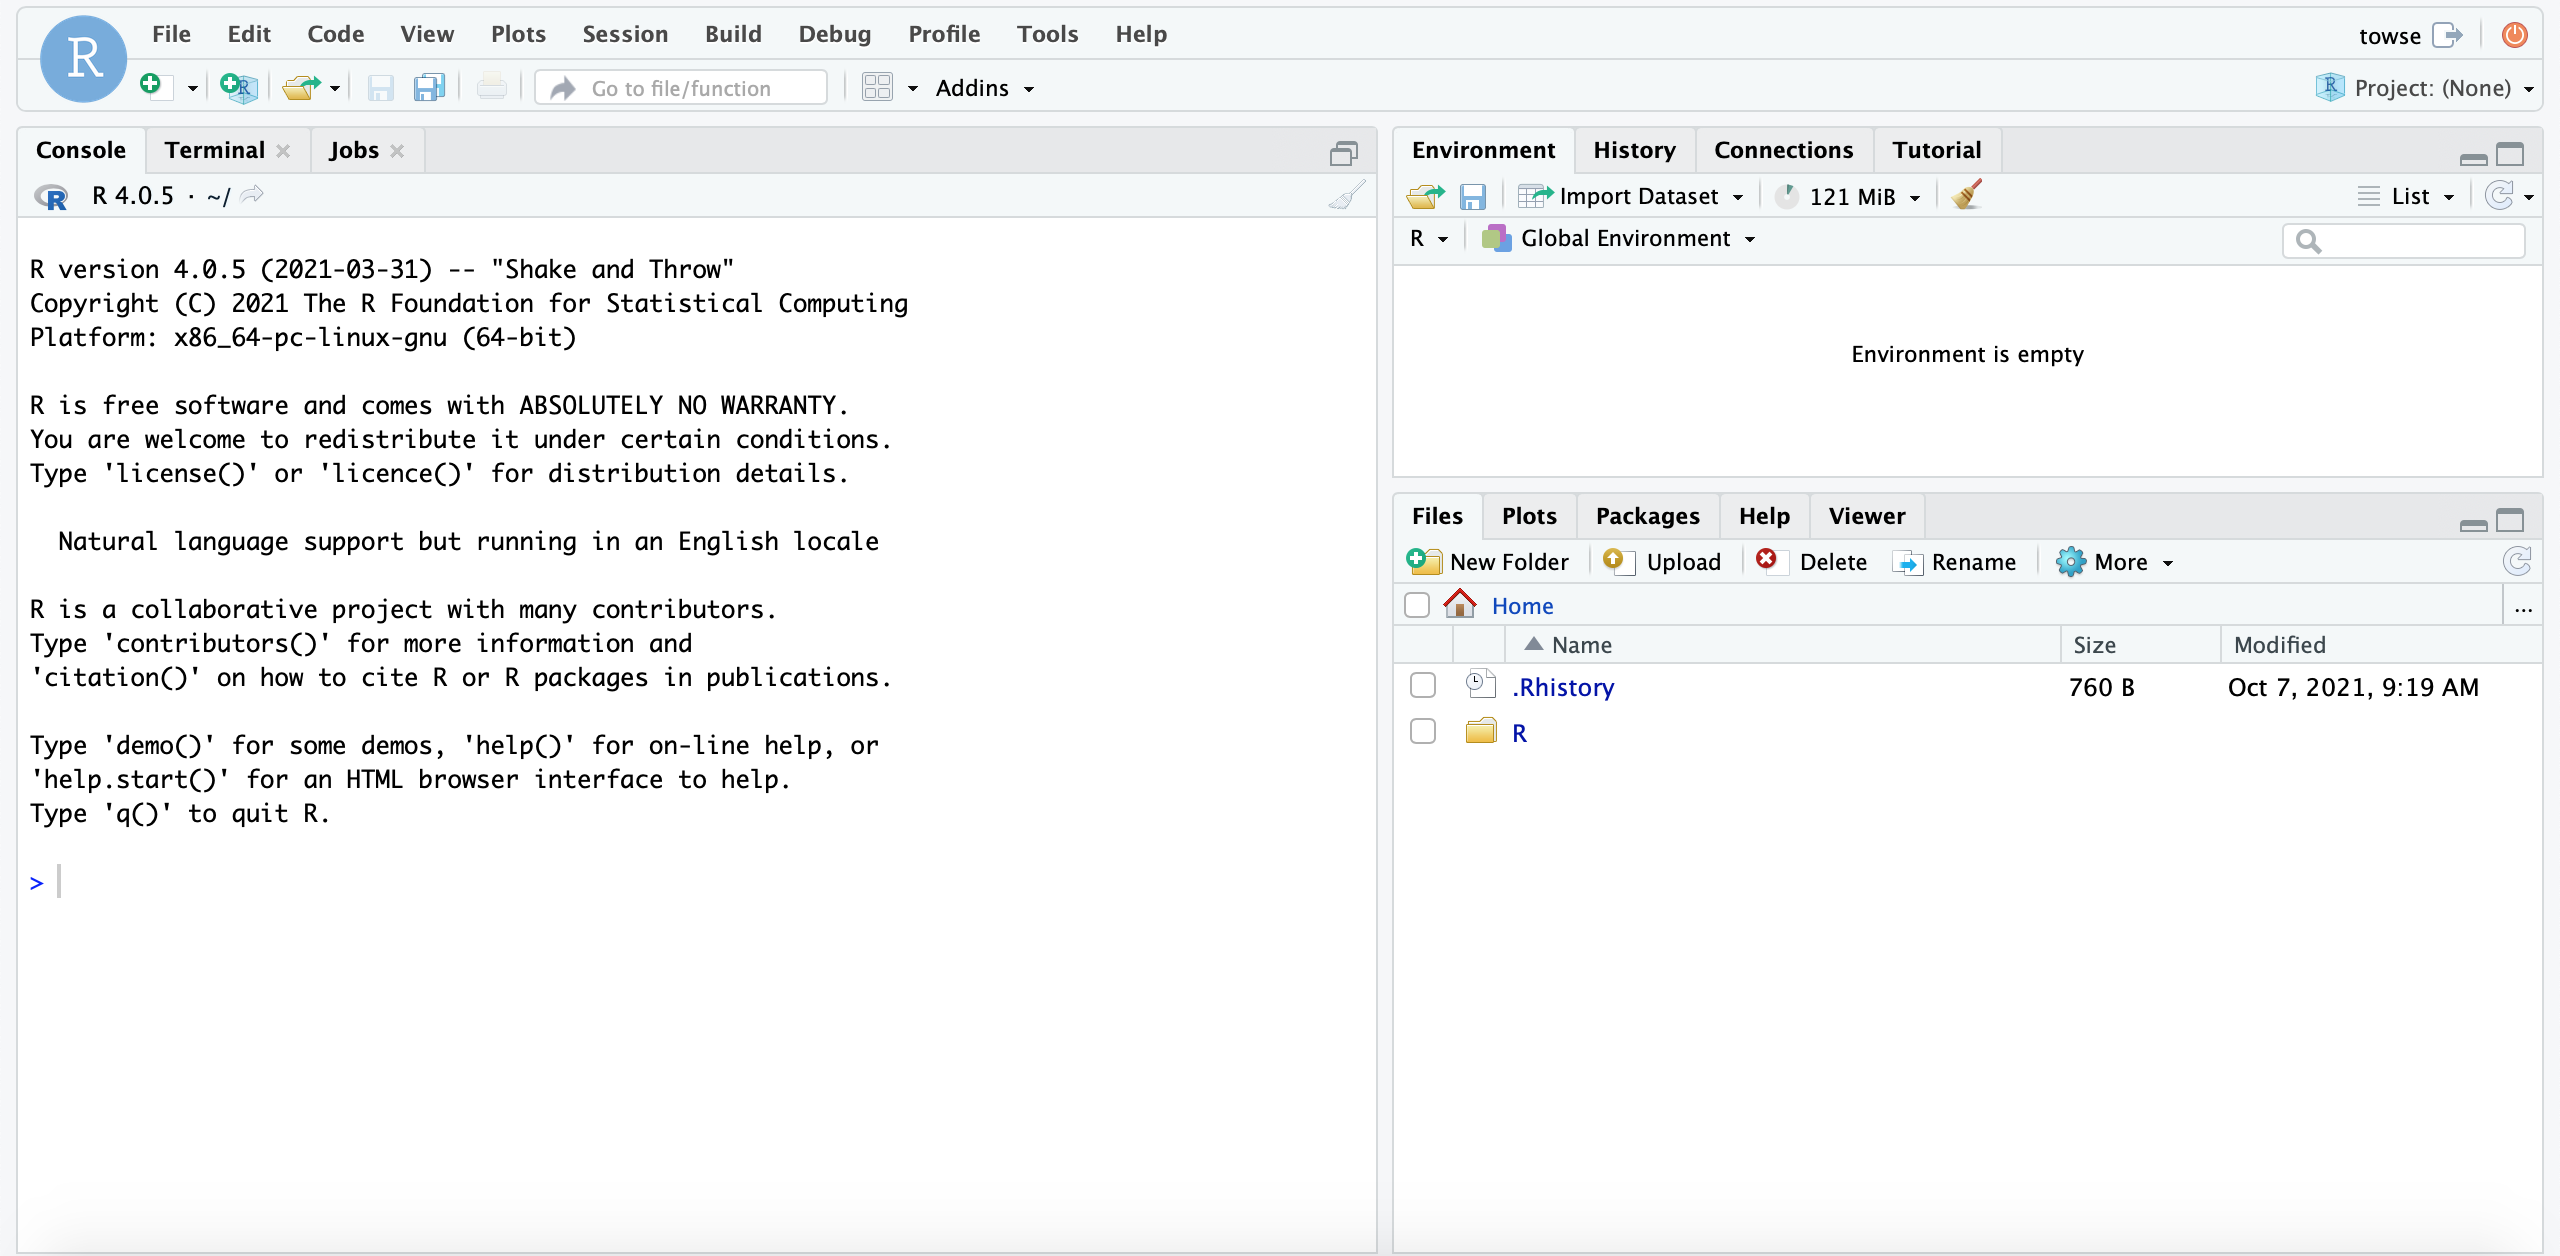
\includegraphics{files/Week_1/server_startup.png}

RStudio has three panels or windows: there are tabs for Console (taking up the left hand side), Environment (and History top right) , Current file (bottom right). You will also see a 4th window for a script or set of commands you develop, also (on the left hand side).

\hypertarget{lets-do-something}{%
\subsection{Let's do something!}\label{lets-do-something}}

In the console window on the left hand side, there's a command prompt ``\textgreater{}''. This is where we ask RStudio to do our bidding!

\begin{enumerate}
\def\labelenumi{\arabic{enumi}.}
\tightlist
\item
  Click in the console window and we will get R to work as a calculator. Type in:
\end{enumerate}

\begin{Shaded}
\begin{Highlighting}[]
\DecValTok{5} \SpecialCharTok{+} \DecValTok{5}
\end{Highlighting}
\end{Shaded}

and press enter. You should get the answer (amazing huh? OK, maybe not \emph{that} amazing\ldots). Use your imagination -- ask a simple arithmetic question of your own choosing!

\begin{enumerate}
\def\labelenumi{\arabic{enumi}.}
\setcounter{enumi}{1}
\tightlist
\item
  In the first analysis lecture, we looked at measures of central tendency and how to calculate them. So let's get R to do these calculations also!
\end{enumerate}

First, we tell R about the data from the lecture. Copy the following line and paste it into the console, then press enter to run it:

\begin{Shaded}
\begin{Highlighting}[]
\NormalTok{PSYC121\_week\_1\_data }\OtherTok{\textless{}{-}} \FunctionTok{c}\NormalTok{(}\DecValTok{7}\NormalTok{,}\DecValTok{8}\NormalTok{,}\DecValTok{8}\NormalTok{,}\DecValTok{7}\NormalTok{,}\DecValTok{3}\NormalTok{,}\DecValTok{1}\NormalTok{,}\DecValTok{6}\NormalTok{,}\DecValTok{9}\NormalTok{,}\DecValTok{3}\NormalTok{,}\DecValTok{8}\NormalTok{)}
\end{Highlighting}
\end{Shaded}

This creates an ``object'' called \texttt{Analysis\_week1\_data}. We can then perform calculations on this object. For example, we can find the mean by using the following command (again, copy and paste)

\begin{Shaded}
\begin{Highlighting}[]
\FunctionTok{mean}\NormalTok{(PSYC121\_week\_1\_data)}
\end{Highlighting}
\end{Shaded}

Check the answer is the same we found in the lecture (it should be 6!).

Next, let's ask for the median:

\begin{Shaded}
\begin{Highlighting}[]
\FunctionTok{median}\NormalTok{(PSYC121\_week\_1\_data)}
\end{Highlighting}
\end{Shaded}

This also should be the answer from the lecture (7)

R doesn't have a single corresponding command for the \emph{mode}, but we can use this series of commands:

\begin{Shaded}
\begin{Highlighting}[]
\NormalTok{getmode }\OtherTok{\textless{}{-}} 
  \ControlFlowTok{function}\NormalTok{(PSYC121\_week\_1\_dataa) \{}
\NormalTok{    uniqv }\OtherTok{\textless{}{-}} \FunctionTok{unique}\NormalTok{(PSYC121\_week\_1\_data)}
\NormalTok{    uniqv[}\FunctionTok{which.max}\NormalTok{(}\FunctionTok{tabulate}\NormalTok{(}\FunctionTok{match}\NormalTok{(PSYC121\_week\_1\_data, uniqv)))]}
\NormalTok{    \}}

\FunctionTok{getmode}\NormalTok{(PSYC121\_week\_1\_data)}
\end{Highlighting}
\end{Shaded}

This is just a bit of clever jiggery-pokery that gets the mode.

\hypertarget{extra-content}{%
\subsection{Extra content}\label{extra-content}}

The commands above are designed to show you that with RStudio active, you can get quick and accurate answers to material covered in PSYC121 lectures.

All we have asked is that you write (or copy in) text to get the information. However, after the lab, you could play around with RStudio in your own time and think about the following:

In R, ``\textless-'' is the assignment operator as in the command we used:

\begin{Shaded}
\begin{Highlighting}[]
\NormalTok{PSYC121\_week\_1\_data }\OtherTok{\textless{}{-}} \FunctionTok{c}\NormalTok{(}\DecValTok{7}\NormalTok{,}\DecValTok{8}\NormalTok{,}\DecValTok{8}\NormalTok{,}\DecValTok{7}\NormalTok{,}\DecValTok{3}\NormalTok{,}\DecValTok{1}\NormalTok{,}\DecValTok{6}\NormalTok{,}\DecValTok{9}\NormalTok{,}\DecValTok{3}\NormalTok{,}\DecValTok{8}\NormalTok{)}
\end{Highlighting}
\end{Shaded}

We create the variable label on the left (\texttt{Analysis\_week1\_data}) and we give it those number on the right. The name \texttt{Analysis\_week1\_data} is largely arbitrary: try use a variable of your own naming (your own name?) instead - and then use that alternative name for the other commands.

\begin{center}\rule{0.5\linewidth}{0.5pt}\end{center}

\textbf{Throughout this year, we'll use the convention of the ``underscore'' to separate words in labels (it\_makes\_them\_easier\_to\_read than ifyoudidn'thaveanyspaces)}

\begin{center}\rule{0.5\linewidth}{0.5pt}\end{center}

What does that tell you about the text used to get the mode? Can you figure out what each line does?

Also, once you have created a variable, you can check what the variable comprises by calling it at the command line. Just write its name, and R will respond with all the data points (all the X values it knows about). Take note that, as you write the variable label, R studio should offer to ``auto-complete'' the name. It only does that if it you have defined the variable, or are writing a known command.

\hypertarget{week-2-descriptive-statistics-in-r-studio}{%
\chapter{Week 2: Descriptive statistics in R Studio*}\label{week-2-descriptive-statistics-in-r-studio}}

\begin{quote}
Written by John Towse \& Tom Beesley
\end{quote}

\hypertarget{pre-lab-work}{%
\section{Pre-lab work}\label{pre-lab-work}}

Last week we asked you to

\begin{itemize}
\tightlist
\item
  Practice a WBA task (the math skill task)
\item
  Connect to the R Studio server and enter some simple commands
\item
  Complete a survey so that we can collect data for analysis teaching
\end{itemize}

This week - we are introducing the \textbf{\texttt{learnr}} tutorial system for lab preparation. This will allow you to try out some useful lab skills before your main lab.

\textbf{Please make sure you've looked at and followed through the exercises here: \url{https://ma-rconnect.lancs.ac.uk/PSYC121_W2_labprep/}}

\hypertarget{file-organisation}{%
\subsection{File organisation}\label{file-organisation}}

We also recommend that you set up your University ``H drive'' by following \href{https://answers.lancaster.ac.uk/display/ISS/Personal+filestore+\%28H+drive\%29+help}{the instructions here}

If you do this, you can organise your files in one place and access them from any university computer that you log in to, including the lab machines in the Levy Lab and the virtual machine (see above). So this effectively acts as a free, cloud-based storage solution for your work (and even personal stuff).

However you choose to store your files, it's essential that you are careful about file organisation. As you progress through these exercises, you will find yourself downloading many data files, and creating many R scripts.

Consider each week a new set of materials that should have it's own folder. Get used to organising your work and you will be well placed to revise the material at a later date.

\hypertarget{r-studio-tasks}{%
\subsection{R Studio tasks}\label{r-studio-tasks}}

For a reminder of how to start R Studio, see the \protect\hyperlink{getting_started}{Week 1 content}.

You can access the RStudio Server at: \url{http://psy-rstudio.lancaster.ac.uk/}

(remember: off campus, you will need to be on the VPN)

\hypertarget{bringing-data-scripts-and-files-into-r-studio}{%
\subsection{Bringing data, scripts and files into R Studio}\label{bringing-data-scripts-and-files-into-r-studio}}

In week 1, we had a tiny dataset that we entered into R through command line. We're going to need a way to tell R about bigger datasets though, so we need to work with datafiles, and bring them into R so that they can form data frames and other forms of data objects in R.

We've provided (on moodle) a walk-though of how to get a data file (in a zip compressed file) into the R environment. Note, once we have imported it into R, it's no longer the original file started with, but within R is has become a named data frame.

\hypertarget{lab-exercises}{%
\section{Lab exercises}\label{lab-exercises}}

\hypertarget{descriptive-information-in-r-studio}{%
\subsection{Descriptive information in R Studio}\label{descriptive-information-in-r-studio}}

Some 5 years ago, a large group of participants gave an estimate of the weight of Penelope the cow. Just over 17,000 guesses. And the distribution of guesses was something like this: 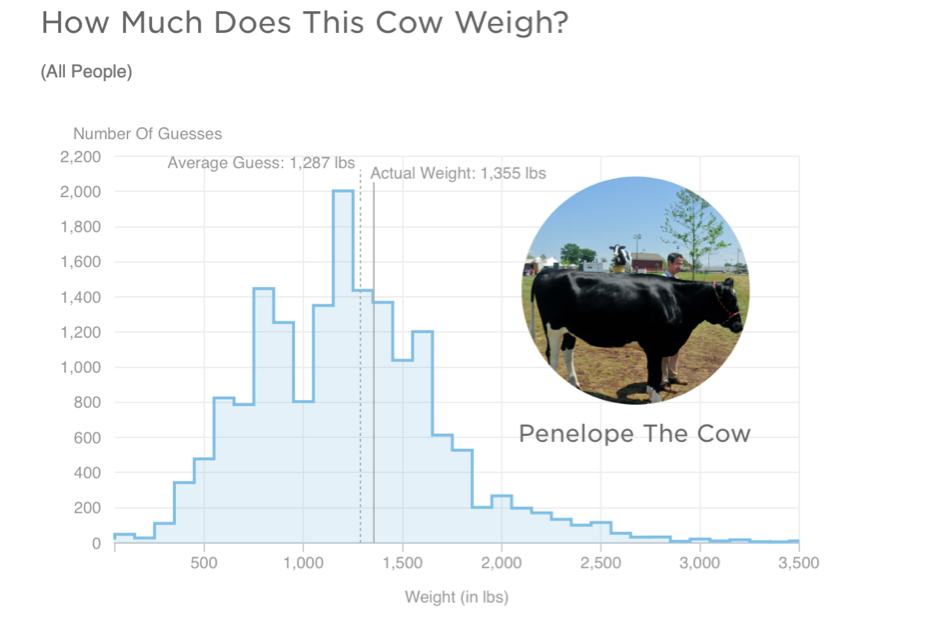
\includegraphics{files/Week_2/penelope.png}

What we can see from this graph is that:

\begin{enumerate}
\def\labelenumi{\arabic{enumi}.}
\tightlist
\item
  Guesses formed a roughly normal distribution. There is a bit of a skew with a right-hand tail, but this is inevitable as a weight of less than 0 is physically impossible, but there is no limit of the semantics of a large guess.
\item
  The mean guess weight (1,287 lbs) is very close to the actual (true) weight of the cow (1,355 lbs). So even though lots of people were inaccurate, a central tendency measure has a pretty good alignment with te true weight. This is known as the Wisdom of Crowds phenomenon, first identified by Galton in 1907 (though he suggested using the median weight)
\end{enumerate}

Let's look at (a smaple of) the PSYC121 student data from 2021 collected on guessing the weight of Penelope, and ask whether it resembles the properties of this large dataset.

\hypertarget{uploading_zip}{%
\subsection{Loading the data}\label{uploading_zip}}

To get the data into R Studio, you need to complete the following steps:

\begin{enumerate}
\def\labelenumi{\arabic{enumi}.}
\tightlist
\item
  Download the ``zip'' file by \href{files/Week_2/Week_2.zip}{clicking this link}
\item
  Find the location of the file on your computer and check it is saved as a ``.zip'' file
\item
  Return to RStudio and navigate to the folder you want to upload the data into (you could create a new folder for this week).
\item
  Click ``Upload''
\item
  Check the target directory is correct
\item
  Click choose file and find the file on your computer.
\item
  Select the file and click ``Open''. Click ``OK''
\end{enumerate}

You should now see the files extracted in the directory. If you receive an ``unexpected server error'' please try this process in a different browser. If you still have trouble, send your username to us \href{mailto:t.beesley@lancaster.ac.uk}{\nolinkurl{t.beesley@lancaster.ac.uk}} for support.

\hypertarget{basic_script}{%
\subsection{Using the R script}\label{basic_script}}

Let's start working with our data, by opening up the ``Week\_2\_script.R'' file. It's part of the zip file for week 2. This is an ``R script'' that contains a series of commands. We could type each of these in the console window (like we did in Week 1), but by having them in a script like this, it saves us typing them or copying and pasting them into the console. It also means we have a record of all the commands we have run.

The first command is to load a library of functions:

\begin{Shaded}
\begin{Highlighting}[]
\FunctionTok{library}\NormalTok{(tidyverse)}
\end{Highlighting}
\end{Shaded}

To run this, simply click anywhere on line 1 of the R script to put the cursor there, and press ctrl+enter (cmd+enter on a mac) or click the button called run. You will see a number of messages appear in the console. Don't worry about these, or worry too much about what exactly this command is doing. Essentially this is giving us some useful tools for our analysis. We will introduce the features of the \textbf{tidyverse} gradually during this course.

(side note: If you were using a local version of R studio on your computer, it might not have the `tidyverse' library already installed. You would need to install the package first)

To import the data into RStudio, from the csv file, simply click the ``Import Dataset'' button in the ``Enviornment'' pane. John has \href{https://dtu-panopto.lancs.ac.uk/Panopto/Pages/Viewer.aspx?id=646a4bd4-9b2e-46a1-b2ee-adc100ce507b}{a video available} to follow along with, if you have trouble with this bit.

The data are in R studio if you have followed all the lab sheet to this point. Note that when you imported the data into the R environment, a command line was generated at the console

\begin{Shaded}
\begin{Highlighting}[]
\NormalTok{ penelope21 }\OtherTok{\textless{}{-}} \FunctionTok{read.csv}\NormalTok{(}\StringTok{"\textasciitilde{}/penelope21.csv"}\NormalTok{)}
\end{Highlighting}
\end{Shaded}

What this command accomplished was to read the spreadsheet called `penelope21' into an object in R called penelope21. You could use any object label, but it's important to then keep that name consistent in what you do next.

The command was also generated

\begin{Shaded}
\begin{Highlighting}[]
 \FunctionTok{View}\NormalTok{(penelope21)}
\end{Highlighting}
\end{Shaded}

which presents the data in a windo of R studio. Note that ``NA'' means not available or missing data. Does this file structure make some sense to you?

\hypertarget{finding-the-mean-and-median-estimates}{%
\subsection{Finding the mean and median estimates}\label{finding-the-mean-and-median-estimates}}

Use the data to answer the following questions\ldots{}

\begin{enumerate}
\def\labelenumi{\arabic{enumi}.}
\tightlist
\item
  What is the mean weight estimates?
\item
  What is the standard deviation of the estimates?
\item
  What is the median weight of the estimates?
\item
  Which of these central tendency measures is the more accurate measure of the true cow weight? (make a judgement)
\item
  What is the mean weight estimate (and standard deviation) for female respondents and non-female (male / non-binary /prefer not to say) respondents?
\end{enumerate}

You may be thinking, how do I possibly do any of this?! Well this week most of the commands you need are contained in the R script you have downloaded. Also, remember from last week, we explored the R command:

\begin{Shaded}
\begin{Highlighting}[]
\FunctionTok{mean}\NormalTok{(lecture1\_data)}
\end{Highlighting}
\end{Shaded}

That gave us the mean of the small dataset ``lecture1\_data''. This time, we want to explore the penelope dataset. But also, the lecture\_data was just a single list of numbers. The penelope21 object is more like a datasheet. So we need to tell R Studio which \textbf{column} we are interested in. RStudio uses the format \textbf{data\$column}. Hence, we can ask

\begin{Shaded}
\begin{Highlighting}[]
\FunctionTok{mean}\NormalTok{(penelope21}\SpecialCharTok{$}\NormalTok{estimate) }
\end{Highlighting}
\end{Shaded}

(this command is in the r script so you don't need to write it out) and to get a standard deviation we can use the command:

\begin{Shaded}
\begin{Highlighting}[]
\FunctionTok{sd}\NormalTok{(penelope21}\SpecialCharTok{$}\NormalTok{estimate)}
\end{Highlighting}
\end{Shaded}

So from this, can you work out what you would do to get the median value (remember from last week how we got the median value?). Part fo the command is given to you, can you change the text so that it works?

\hypertarget{calculations-from-a-range-of-columns}{%
\subsection{Calculations from a range of columns}\label{calculations-from-a-range-of-columns}}

We have seen that:

\begin{Shaded}
\begin{Highlighting}[]
\FunctionTok{mean}\NormalTok{(penelope21}\SpecialCharTok{$}\NormalTok{estimate) }
\end{Highlighting}
\end{Shaded}

will provide a mean of the column ``estimate''. In the third column, named ``female\_estimate'', we have the estimates of just the female respondents. In the fourth column, named ``other\_estimate'', we have the estimates of the ``other'' respondents (males and non-binary and prefer not to say).

So can you now figure out how you might get information about the estimate from the female data (only) or the non-female data? Try it, based on what you have just done. Does it work?

You will find that the result of the this command produces an ``NA'' result. This means that the answer is ``Not Available'', or in other words, is a ``missing value''. This is because some of the values in this column are NA, and the mean of a column with NAs will always lead to the result NA.

Instead, try this command:

\begin{Shaded}
\begin{Highlighting}[]
\FunctionTok{mean}\NormalTok{(penelope21}\SpecialCharTok{$}\NormalTok{female\_estimate, }\AttributeTok{na.rm =} \ConstantTok{TRUE}\NormalTok{ )}
\end{Highlighting}
\end{Shaded}

Any different? The \texttt{na.rm\ =\ TRUE} instruction tells RStudio that missing data can be ignored in this mean calculation. (in technical language, \texttt{na.rm} is a parameter of the function \texttt{mean} that removes the NAs if set to TRUE)

\hypertarget{simple-graphs}{%
\subsection{Simple graphs}\label{simple-graphs}}

RStudio can be used to create graphical data plots that can help interpret datasets

The first thing we can do is create a histogram distribution of guesses from the sample student data to compare with the previous large sample study (i.e.~the 17,000 guesses):

\begin{Shaded}
\begin{Highlighting}[]
\FunctionTok{hist}\NormalTok{(penelope21}\SpecialCharTok{$}\NormalTok{estimate)}
\end{Highlighting}
\end{Shaded}

We can also create a ``box and whisker plot''. Here's a general simple description of a box-and-whisker plot as a graphical representation of data:

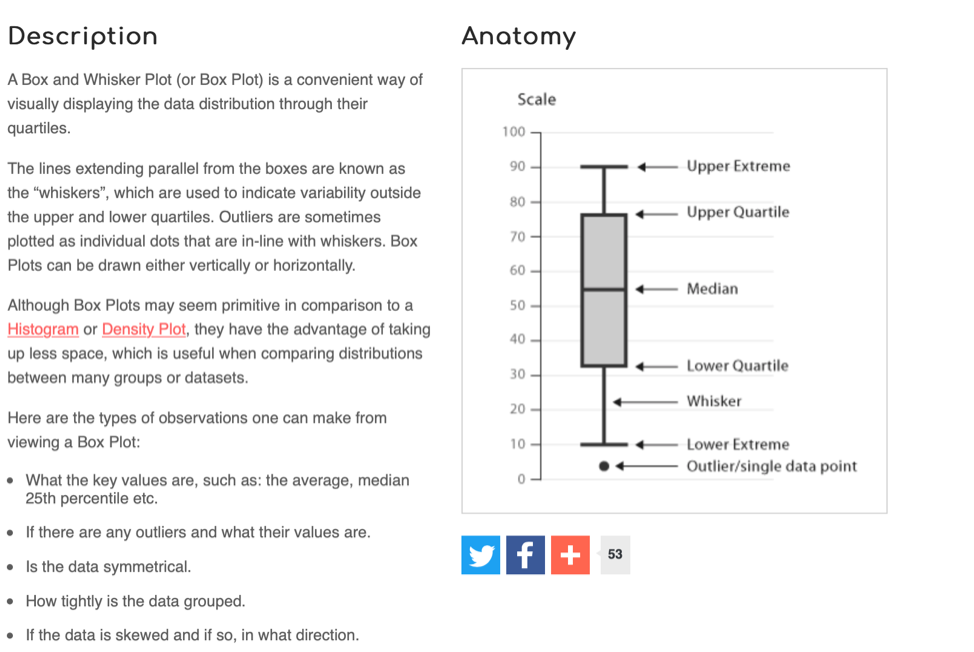
\includegraphics{files/Week_2/Box_and_whisker.png}

We can create a box and whisker plot for the estimate column using the following command:

\begin{Shaded}
\begin{Highlighting}[]
\FunctionTok{boxplot}\NormalTok{(penelope21}\SpecialCharTok{$}\NormalTok{estimate)}
\end{Highlighting}
\end{Shaded}

\hypertarget{extra-content-1}{%
\section{Extra content!}\label{extra-content-1}}

Want to try explore some more outside of the analysis class before next week and improve your R skillset? Try these exercises:

\hypertarget{helping-yourself}{%
\subsection{Helping yourself!}\label{helping-yourself}}

If you're not sure how a command works, or some detail of command, then R itself may be able to help you. You can ask for help for example by entering the command

help(mean)

Try get help on other commands we have explored this week. Does the help info converge with your growing knowledge of the commands? Does the help show you some of the additional options with the commands? Can you use the examples which may accompany the help info?

You can also use help() to find out more about packages rather than just commands (see next challenge). And most help info will give some example, but you can ask for examples specifically with example() (e.g.~example(mean))

\hypertarget{create-a-box-and-whisker-plot-of-both-the-female-and-non-female-data-on-the-same-figure.}{%
\subsubsection{Create a box-and-whisker plot of BOTH the female and non-female data on the same figure.}\label{create-a-box-and-whisker-plot-of-both-the-female-and-non-female-data-on-the-same-figure.}}

To do so, you can use a really flexible toolkit (in R-speak, called a package) with publisher-quality graphics capabilities called ``ggplot2''. We turned this on with the command before

\begin{Shaded}
\begin{Highlighting}[]
\FunctionTok{library}\NormalTok{(tidyverse)}
\end{Highlighting}
\end{Shaded}

Have a look at the help information about for example, ``geom\_boxplot'', and try out the script information provided for week 2. The challenge is to figure out how the script instructions produce the graph -- what do the elements do (maybe fiddle around with it to find out!).

Good luck!

\hypertarget{week-3-dvs-and-ivs-in-r-studio}{%
\chapter{Week 3: DVs and IVs in R Studio}\label{week-3-dvs-and-ivs-in-r-studio}}

\begin{quote}
Written by John Towse \& Tom Beesley
\end{quote}

\hypertarget{pre-lab-work-1}{%
\section{Pre-lab work}\label{pre-lab-work-1}}

Last week we asked you to

\begin{itemize}
\tightlist
\item
  Complete the teaching dataset survey
\item
  Prepare for the lab class with the learnr tutorial
\item
  Complete some R Studio exercises working with data and a script to get some descriptives and some data
\end{itemize}

This week - again, there's a learnr tutorial to follow and help prep for this week's activties : \url{https://ma-rconnect.lancs.ac.uk/W3_LabPrep/}

About 1/3 of students at the time of writing this had yet to complete the teaching survey. We'd really appreciate more completions so we can work with a good sample of data this term, and as a reminder, the data are here: \url{https://lancasteruni.eu.qualtrics.com/jfe/form/SV_6rLPbl1YI8Y2WXj}

Since we've got less data than we would expect, we can't yet use the data in this term's activities.

\hypertarget{r-studio-tasks-1}{%
\section{R Studio tasks}\label{r-studio-tasks-1}}

For the ``penelope21'' data in week 2, we provided you with estimates data, and you were able to generate descriptive statistics for the estimates (if not, please go back and work through that part of the week 2 lab sheet again). You also found the weight estimates for the female and non-female guesses, right?

However, in order to find the estimates separately for gender identity, we needed to have a column for each gender category. Whilst that worked, it could get cumbersome over time always to work with data created like that.

\emph{There is a better way}

\hypertarget{task-1---penelope21-data}{%
\subsection{Task 1 - penelope21 data}\label{task-1---penelope21-data}}

Download the \href{files/Week_3/Week_3.zip}{week3.zip} file and upload it into R Studio server. If you need them, \protect\hyperlink{uploading_zip}{here are the key instructions} from Week 2.

Import the ``penelope21'' data using the \texttt{read.csv()} command (if unsure, see here in \protect\hyperlink{basic_script}{Week 2}), and launch the R script.

This week, we want to explore commands from the tidyverse library (toolkit) which can help us do more powerful things more elegantly. So let's get R to work with the tidyverse library

\texttt{library(tidyverse)}

(Nb. This command is the accompanying R script. You can access it from there.)

This time, let's ask for the estimate data arranged by identity:

\texttt{aggregate(x\ =\ penelope21\$estimate,\ by\ =\ list(penelope21\$identity),\ FUN\ =\ mean)}

First, let's try this! What do you get? Does this match what we did last week when we calculated the mean for the female and for the other group?

Second, let's look at what is happening here:

\texttt{aggregate} This is a command to get descriptive statistics
Remember we can use help to find more about this command!

\texttt{x=}~\\
This defines what column we are analyzing

\texttt{by=list}~\\
Now we tell R how to group the estimate data, and which column does that

\texttt{FUN=mean}~\\
Specifies which descriptive function is being asked for
Can you explore whether you can call on alternate measures?)

\hypertarget{group_by}{%
\subsection{group\_by()}\label{group_by}}

There's another way that also allows us to group scores by a (nominal) variable. This is explored in the learnr tutorial, which should help you create the command the get weight estimates broken down by gender identity. You need to define the data frame for the estimates data, and the gender IV and the estimates DV

\texttt{*MISSING*\ \%\textgreater{}\%\ group\_by(*MISSING*)\ \%\textgreater{}\%\ summarise(mean\_estimate\ =\ mean(*MISSING*))}

First, try this command and see what you get. If you run this command as entered, it won't work. So now use your experience at skills from the above and the learnr tutorial to work out what is required.

Note

\texttt{\%\textgreater{}\%}~\\
This is a ``pipe operator'', basically take the output from the left and feed it into the requests on the right. \texttt{Summarise}\\
Provide summary statistics information for the specified variable as specified (whether mean, median etc)

\hypertarget{the-assignment-operator}{%
\subsection{The assignment operator}\label{the-assignment-operator}}

As well as learning about the pipe operator, we want to introduce another important element of the R command line syntax: the assignment operator.

Probably without knowing about it, we've been using this already! When a dataset is imported into R Studio from the menu, a command is created such as

penelope21 \textless- read.csv(``\textasciitilde/penelope21.csv'')

What this does is look for the csv datafile called `penelope21', and assign it to an object / variable called `penelope21'

We could create any object name we wanted (within limits of names already known to R Studio). If we wanted to work with something called ``week\_3\_data'' we could use

week\_3\_data \textless- read.csv(``\textasciitilde/penelope21.csv'')

In R Studio, we would call on ``week\_3\_data'' rather than ``penelope21'' in the command lines.

\hypertarget{task-2---salary20-data}{%
\subsection{Task 2 - Salary20 data}\label{task-2---salary20-data}}

Using aggregate and summarise may not seem like much progress, because they are just replicating what we had already done with mean() is week 2. However (a) this emphasizes that there are often several ways to get at the same thing in R (b) now we know about grouping, we can start to do more efficient and informative things.

Now, let's turn to the guesses made about median salary in the UK. We can get the data (created in 2020) from the file ``salary20'' in the week 3.zip file;

Let's take a peek at the dataset with

\texttt{glimpse(salary20)}

Glimpse pretty much does what you might think from the meaning of the word -- it just gives us a data sample (handy because this is a much bigger dataset) and shows that we have 3 columns; UK\_region (where someone lives, note `other' probably equals Northern Ireland, Europe, China, etc, family\_position (age relationship with siblings), and median\_salary guess.

By the way, the govt statistics say the actual median income in 2019 was approx. £30,350 \url{https://www.statista.com/statistics/1002964/average-full-time-annual-earnings-in-the-uk/}

\begin{enumerate}
\def\labelenumi{\Alph{enumi})}
\tightlist
\item
  Can you use the ``aggregate'' command from task 1 to find out the salary guesses as a function of where someone lives? That is, can you adapt that code for this problem?
\item
  Can you use the aggregate command to find out salary guess as a function of family relationships? (if you are the youngest child maybe you have older siblings earning money that changes your evaluation?)
\item
  Can you get a breakdown of guess as a function of BOTH UK region AND family relationship together?
\item
  Can you adapt the ``summarise'' command to display salary guesses as a function of where someone lives?
\item
  Use R Studio to figure out the overall mean salary estimate and the standard deviation. Calculate by hand what salary estimate would have a z score of z=-1.5?
\end{enumerate}

\hypertarget{week-4-z-score-calculations-and-dvsivs-again}{%
\chapter{Week 4: Z-score calculations and DVs/IVs again}\label{week-4-z-score-calculations-and-dvsivs-again}}

\begin{quote}
Written by John Towse \& Tom Beesley
\end{quote}

\hypertarget{pre-lab-work-2}{%
\section{Pre-lab work}\label{pre-lab-work-2}}

This week - again, there's a learnr tutorial to follow and help prep for what we are covering: \url{https://ma-rconnect.lancs.ac.uk/W4_LabPrep/}

\hypertarget{r-studio-tasks-2}{%
\section{R Studio tasks}\label{r-studio-tasks-2}}

Last week we introduced two different ways to get a variable / column of scores investigated as a function of a separate column of data. In others words, describe the DV a function of an IV

Those two approaches involved

\texttt{aggregate(x\ =\ DV,\ by\ =\ list(IV),\ FUN\ =\ mean)}

and

\texttt{data.frame\ \%\textgreater{}\%\ group\_by(IV)\ \%\textgreater{}\%\ summarise(mean\_estimate\ =\ mean(DV))}

Use the \href{https://ma-rconnect.lancs.ac.uk/W3_LabPrep/}{week 3 learnr tutorial} from last week to get more hints and practice with this, if you need to, alongside the week 4 tutorial.

\hypertarget{task-1---climate-change-data}{%
\subsection{Task 1 - Climate change data}\label{task-1---climate-change-data}}

\begin{enumerate}
\def\labelenumi{\arabic{enumi}.}
\tightlist
\item
  Download the \href{files/Week_4/Week_4.zip}{week4.zip} file and upload it into R Studio server. If you need them, \protect\hyperlink{uploading_zip}{here are the key instructions} from Week 2. This week the data is called ``climate''. Launch the week\_4 R script as before.
\end{enumerate}

Step 2. Once again, we're gong to be using commands from the tidyverse library (the pipe operator is one example) so we need to ensure that it's active. Run the command:

\texttt{library(tidyverse)}

(Nb. This command is the accompanying R script. You can access it from there.)

In the climate data frame, there are the following variables:

\emph{human\_CC} - A response to the question: How much do you think human activity contributes to climate change, as a percentage of overall climate change? Please enter a value between 0 (humans do not contribute to climate change at all) and 100 (human contribute entirely to climate change).

\emph{UK\_region} - where in the UK you used to live

\emph{country\_visits} - the number of countries you have visited

\emph{visit\_category} - a number between 1-3

\begin{itemize}
\item
  1 means you have visited 1-4 countries
\item
  2 means you have visited 5-9 countries
\item
  3 means you have visited more than 9 countries
\end{itemize}

Step 3. Maybe belief in human activity as a contributor to climate change varies across the UK? Find out which region of the UK has the highest and the lowest belief in the relative role of human activity in climate change. Change the following command based on what was learnt last week and the current data described above

\texttt{Data\_frame\_name\ \%\textgreater{}\%\ group\_by(IV)\ \%\textgreater{}\%\ summarise(mean\_estimate\ =\ mean(DV))}

Step 4. Maybe views about climate change are affected by how well travelled you are? Because you see the global impacts of clmate change, or because travel (often producing carbon emissions) is a sign of not being worried. So use the climate\_change\_category to look at whether there are differences in rating of human contribution to climate change.

\hypertarget{extra-activity.}{%
\subsection{Extra activity.}\label{extra-activity.}}

Come back to this afterwards for some extra practice if you want: Use the learnr activities to think about visualisation of the climate data. What graph(s) would be useful? How can you customise them?

\hypertarget{z-scores}{%
\section{Z-scores}\label{z-scores}}

\begin{quote}
Hint / Reminder: Sketch a normal (z score) distribution and mark the mean/mode, and mark off the relevant parts of the question so you know what you are trying to achieve and how to interpret any calculations you make.
\end{quote}

\begin{quote}
Hint/ Reminder 2. For questions 6 \& 7, remember that from the week 4 lecture material, typically in psychology we use the 5\% level as a cutoff to decide, in broadly described terms, whether something is extreme or unlikely vs.~at least somewhat plausible or likely.
\end{quote}

\hypertarget{z-scores-1-distributions}{%
\subsection{z-scores 1: distributions}\label{z-scores-1-distributions}}

Q1. What is the relationship between the sign of a z-score and its position in a distribution?

Q2. If a distribution has a mean of 100 and a standard deviation of 10, what is the raw score equivalent to a z-score of 1.96?

Q3. If a distribution has a mean of 157 and a standard deviation of 19, what is the raw score equivalent to a z-score of 1?

\hypertarget{z-scores-2-using-z-score-tables}{%
\subsection{z-scores 2: Using z-score tables}\label{z-scores-2-using-z-score-tables}}

Q4. What proportion of scores lie between the mean and a z-score of 0.5?

Q5. What is the combined proportion of scores lying between z=-1.2 and z=.85?

\hypertarget{z-scores-3-applying-z-scores-to-inferential-problems}{%
\subsection{z-scores 3: Applying z-scores to inferential problems}\label{z-scores-3-applying-z-scores-to-inferential-problems}}

Q6. A Neuropsychologist has presented a test of face recognition to 200 neurotypical participants and finds that the scores are normally distributed with a mean of 85 and the standard deviation of 12. Two brain-damaged patients are also given the test. The one with right hemisphere brain damage scored 58 and the one with left hemisphere damage scored 67.

\begin{enumerate}
\def\labelenumi{\arabic{enumi}.}
\item
  What is the z score of the right hemisphere patient when compared to the neurotypical group?
\item
  What proportion of neurotypical participants score lower that this patient?
\item
  Is this patient likely to belong to the population of neurotypical participants? (justify your answer)
\item
  What is the z score of the left hemisphere patient when compared to the neurotypical group?
\item
  What proportion of neurotypical participants score lower than this patient?
\item
  Is this patient likely to belong to the population of neurotypical participants? (justify your answer)
\end{enumerate}

\hypertarget{extra-activity}{%
\subsection{Extra activity}\label{extra-activity}}

Come back to this afterwards for some extra practice if you want:

Q7. Tim Bizzley has measured the foot size of men and women and found each to be normally distributed. The men have a mean size of 55 with a standard deviation of 5 and the women a mean of 33 and a standard deviation of 5. Joanna Toes has foolishly measured two individuals but forgotten to note their gender. These have foot sizes of 37 and 47. To which gender is each more likely to belong? What evidence is there for this?

\hypertarget{week-6-visualising-data-and-binomial-tests}{%
\chapter{Week 6: Visualising data and binomial tests}\label{week-6-visualising-data-and-binomial-tests}}

\begin{quote}
Written by Tom Beesley \& John Towse
\end{quote}

They say a picture paints a thousand words, so in this week's lab we will be learning some fundamental skills in \textbf{data visualisation} with the \texttt{ggplot()} commands. We will then conduct our first statisitical test to tell whether there is a \emph{real difference} in our data. You must ensure you have watched the lecture and done the pre-lab work before coming to class.

\hypertarget{pre-lab-work-online-tutorial}{%
\section{Pre-lab work: online tutorial}\label{pre-lab-work-online-tutorial}}

To access the \href{https://ma-rconnect.lancs.ac.uk/Week_6_LabPrep}{\textbf{pre-lab tutorial click here}} (on campus, or VPN required)

\hypertarget{rstudio-task-1-creating-a-new-folder-and-project}{%
\section{RStudio Task 1: Creating a new folder and project}\label{rstudio-task-1-creating-a-new-folder-and-project}}

We are going to set up a new folder for this week and an RStudio \emph{Project}. This is a good practice for organising your scripts and data.

\begin{enumerate}
\def\labelenumi{\arabic{enumi}.}
\tightlist
\item
  When you are logged on to the \href{http://psy-rstudio.lancaster.ac.uk}{\textbf{RStudio Server}}, navigate to your home directory by clicking on the small house icon:
\end{enumerate}

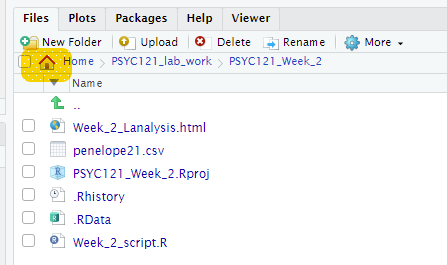
\includegraphics{files/Week_6/home_button.png}

\begin{enumerate}
\def\labelenumi{\arabic{enumi}.}
\setcounter{enumi}{1}
\item
  Click the ``New Folder'' button just above the home button. Name the folder something sensible (e.g., Week\_6) and click OK.
\item
  Click on this folder and then click ``More'' and ``Set As Working Directory''. This tells RStudio that you are now working in this directory. When you read in data using \texttt{read.csv} it will know where to look for the file name that you provide.
\end{enumerate}

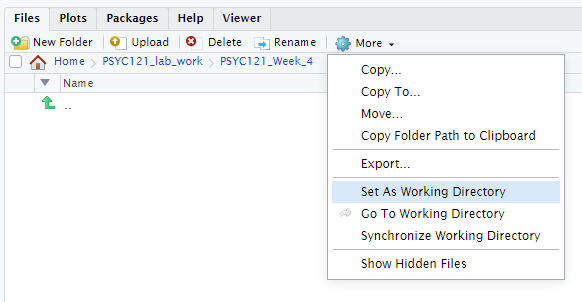
\includegraphics{files/Week_6/working_dir.png}

\begin{enumerate}
\def\labelenumi{\arabic{enumi}.}
\setcounter{enumi}{3}
\item
  Let's add the files we need for this week. Download the \href{files/Week_6/Week_6.zip}{Week\_6.zip} and upload it into RStudio Server. If you need them, \protect\hyperlink{uploading_zip}{here are the key instructions} from Week 2.
\item
  Now let's finish this process by making this a \emph{Project}. Click on the small blue icon in the top right of RStudio, and clicking ``New Project'':
\end{enumerate}

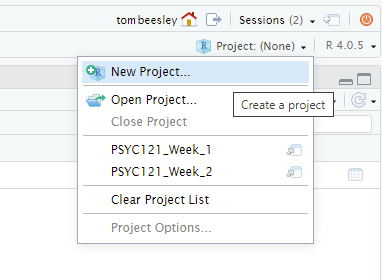
\includegraphics{files/Week_6/new_project.png}

\begin{enumerate}
\def\labelenumi{\arabic{enumi}.}
\setcounter{enumi}{5}
\item
  You may be asked to save the workspace or data - you should do this. Then select ``Existing Directory'' and make sure that the new directory you have created is selected as the ``Project Working Directory'' - it should be, if you set the working directory correctly above. If not, navigate to the correct directory here.
\item
  And you're done! This should now appear as a project in your front page on RStudio. You can get back to that front page by clicking the red power button in the top right corner. Using projects has many benefits. It will keep all the content for the week in one place, and save the commands you've used in the console. You can also use the \emph{Project Menu} to navigate quickly between different projects.
\end{enumerate}

\hypertarget{rstudio-task-2-visualising-phone-use}{%
\section{RStudio Task 2: Visualising phone use}\label{rstudio-task-2-visualising-phone-use}}

It's time to put the skills you learnt in the online tutorial into practice with a new data set. In the survey, people estimated their daily phone use, and then looked up the actual time their phones were on. This data is provided in the zip file.

\begin{enumerate}
\def\labelenumi{\arabic{enumi}.}
\item
  Open the script ``Week\_6\_script.R''. This is the script file you will use for this task and the next one (3).
\item
  Run the first two lines of code \texttt{library(tidyverse)} and \texttt{data\_w6\ \textless{}-\ read\_csv("data\_phone.csv")}. Note that the \texttt{read\_csv()} function is another way to import data. A shortcut version of using the ``Import Dataset'' action.
\item
  You should now have an object in environment called \texttt{data\_w6}. You can view this (the ``spreadsheet view'') by clicking on the object.
\item
  Try running the ggplot command. You will see that this generates an error in red. Oh no!! Don't panic. Look at what it's telling you is wrong. Let's look at the ggplot command and edit it to make it display something. As a reminder from the online tutorial:
\end{enumerate}

\begin{quote}
The main graphing command is \texttt{ggplot()} which tells R we want to draw some kind of plot. If you want to, you can just run \texttt{data\_w6\ \%\textgreater{}\%\ ggplot()}, and you'll see that R produces just a blank plot window. The plot is blank because we haven't told it a) what type of plot we want, and b) what data to plot.
\end{quote}

\begin{quote}
Note that the next line is \textbf{added} to \texttt{ggplot()} (i.e., \texttt{ggplot()\ +\ geom\_point()}). Plotting with \texttt{ggplot()} involves adding elements (geoms) together. Think of it as adding layers on top of each other: the ggplot() is your pizza base, and the geoms and other features are the toppings!
\end{quote}

\begin{quote}
Within the \texttt{geom\_point()} command we have the very important command of \texttt{aes()}. This stands for \textbf{aesthetics}. \texttt{aes()} tells ggplot how the data should be represented on the features of the plot.
\end{quote}

\begin{enumerate}
\def\labelenumi{\arabic{enumi}.}
\setcounter{enumi}{4}
\item
  Add y and x components inside the \texttt{aes()} command. These are used to map variables in your data to the features of the graph. If you are stuck on this, it's time to go back and look at the
\item
  Inside the \texttt{aes()} command, map the variable \emph{screen\_time\_estimate} to the x axis, and the variable \emph{screen\_time\_actual} to the y axis. In general, does it look like people's estimates were accurate?
\item
  Add a setting for \emph{colour} outside of the \texttt{aes()}, to make all the points red. Why outside of \texttt{aes()}? Well remember from the online tutorial:
\end{enumerate}

\begin{quote}
Careful observation of the code here will show you that these new commands are written \textbf{outside} of the \texttt{aes()} command. This is really important to note. We write these outside of \texttt{aes()} because these features of the plot \textbf{are not related to the data}. We are NOT \emph{mapping} any of our data to these features. Instead, we are simply specifying one particular value for each of these ``settings'' in the plot
\end{quote}

\begin{enumerate}
\def\labelenumi{\arabic{enumi}.}
\setcounter{enumi}{7}
\item
  Now map the \emph{colour} to the variable \emph{phone\_type} (within \texttt{aes()}). Can you see any differences between people who have different phones?
\item
  Try changing your \texttt{geom\_point()} command to \texttt{geom\_jitter()} (keeping the mappings the same). Suddenly this reveals many more points! Why is this? Check the help to find out more about this geom: \texttt{?geom\_jitter}.
\end{enumerate}

\hypertarget{rstudio-task-3-conducting-a-binomial-test}{%
\section{RStudio Task 3: Conducting a binomial test}\label{rstudio-task-3-conducting-a-binomial-test}}

Let's now look at whether these differences we see are meaningful. Do people estimate their daily screen time to be more than it actually is? There are two blocks of code to run here. You don't have to edit these, but it's important to look at what they are doing:

\begin{enumerate}
\def\labelenumi{\arabic{enumi}.}
\item
  Run the first block of code. This adds a new column to the data, \emph{est\_diff}, which means the ``estimate difference'': actual screen time minus estimated screen time. You can take a look at this code by clicking on the new object in the environment, \emph{data\_phone\_diff}. What do the positive and negative values reflect?
\item
  Run the second block of code. This filters out (!= means ``not equal to'') the zero values in the est\_diff column. Why is this important for the sign test?
\item
  The result of the final line of code (\texttt{count()}) will be output in the console. This tells us how many values were above 0 (TRUE) and how many below zero (FALSE). This is all the information we need to conduct our statistical test:
\end{enumerate}

\begin{itemize}
\tightlist
\item
  How many positive values were there (above 0)?.
\item
  How many observations were there in total?
\item
  Add these two values to the two ``MISSING'' values in code for the binomial test
\item
  Run the test and read the output - and take note of the ``p-value''
\item
  This tells us how likely such a result would be if the null hypothesis was true.
\item
  Does this mean there is a significant over or underestimate in people's estimates of phone time usage?
\end{itemize}

\hypertarget{extra-content-2}{%
\section{Extra content!}\label{extra-content-2}}

Visualising data is all about communication: how can I communicate my results so that it makes the data very easy to interpret. Try these additional steps:

\begin{enumerate}
\def\labelenumi{\arabic{enumi}.}
\item
  Add a \texttt{labs()} layer to modify text on the graph. If you're not sure how to do this, then feel free to go back to the online tutorial, or take a look at the help wiht \texttt{?labs}. Try changing the axis titles and add a title for the graph.
\item
  Change the theme of the graph. Try \texttt{?theme\_classic} for help.
\item
  Graphs can be saved by clicking \emph{Export}, then \emph{Save as image}. Set the dimensions to how you like it to look, give it a suitable filename, and click save.
\end{enumerate}

\hypertarget{week-7-draft---do-not-complete-yet-one-sample-t-test-on-salary-estimates}{%
\chapter{Week 7: {[}DRAFT - do not complete yet{]} One-sample t-test on salary estimates}\label{week-7-draft---do-not-complete-yet-one-sample-t-test-on-salary-estimates}}

\begin{quote}
Written by Tom Beesley \& John Towse
\end{quote}

Today we will look in a bit more detail at people's estimates of the average UK salary. We will first plot this data using continue to develop our skills in \textbf{data visualisation} with the \texttt{ggplot()} commands. We will look at plotting means and standard errors, and at how geoms can share aesthetic mappings. We will explore our data on the famous ``Stroop Task'' and calculate

\hypertarget{pre-lab-work-online-tutorial-1}{%
\section{Pre-lab work: online tutorial}\label{pre-lab-work-online-tutorial-1}}

\textbf{Online tutorial}: To access the \href{https://ma-rconnect.lancs.ac.uk/Week_7_LabPrep}{\textbf{pre-lab tutorial click here}} (on campus, or VPN required)

\textbf{Getting ready for the lab class}

\begin{enumerate}
\def\labelenumi{\arabic{enumi}.}
\item
  Create a folder and a Project for Week 7. \protect\hyperlink{creating_project}{Click here for the instructions} from last week if you are unsure.
\item
  Download the \href{files/Week_7/Week_7.zip}{Week\_7.zip} and upload it into this new folder in RStudio Server. If you need them, \protect\hyperlink{uploading_zip}{here are the instructions} from Week 2.
\end{enumerate}

\hypertarget{rstudio-task-1-plotting-and-filtering}{%
\section{RStudio Task 1: Plotting and filtering}\label{rstudio-task-1-plotting-and-filtering}}

\textbf{Important!} - You should be using the Week\_7\_script as you work through these tasks. Edit the script to complete the tasks. Running code from the script is easy - place your cursor on the line or block of code you want to run and press ``run'' (of ctrl/cmd+enter). See the video on Moodle if you're unsure.

\begin{enumerate}
\def\labelenumi{\arabic{enumi}.}
\item
  Open the Week\_7\_script and run the \texttt{library} and \texttt{read\_csv} commands
\item
  Complete the \texttt{geom\_histogram()} code to plot the distribution of salary data
\item
  OK - we've got some pretty funky values here! Some people think the average salary is £500,000!!! Well, maybe they just added too many zeros (let's give them the benefit of the doubt). Run the \texttt{arrange()} code to see what those high values are.
\item
  We'll need to remove these high values to get a better sense of the distribution. Let's use a \texttt{filter()} command to do this. Edit the \texttt{filter()} command to keep only those estimates that are below £200,000. Note that you are making a new object at this step (\emph{data\_w7\_f}).
\item
  Now your filter has done its job, let's plot the data again. Edit the \texttt{aes()} command to draw the histogram.
\item
  And as you know, we can also look at the distribution as a boxplot. Edit the \texttt{geom\_boxplot()} code to do this.
\end{enumerate}

\hypertarget{testing-if-the-effect-is-significant}{%
\subsection{Testing if the effect is significant}\label{testing-if-the-effect-is-significant}}

We now want to know if the salary estimates are different to the actual average salary in the UK (which is approx. £30,000).

\begin{enumerate}
\def\labelenumi{\arabic{enumi}.}
\setcounter{enumi}{6}
\item
  First, let's calculate the \texttt{mean()} of our salary estimates.
\item
  Now we can compute a t-statistic. Edit the code on this line to conduct a one-sample t-test\ldots{[}more interpretation here{]}
\end{enumerate}

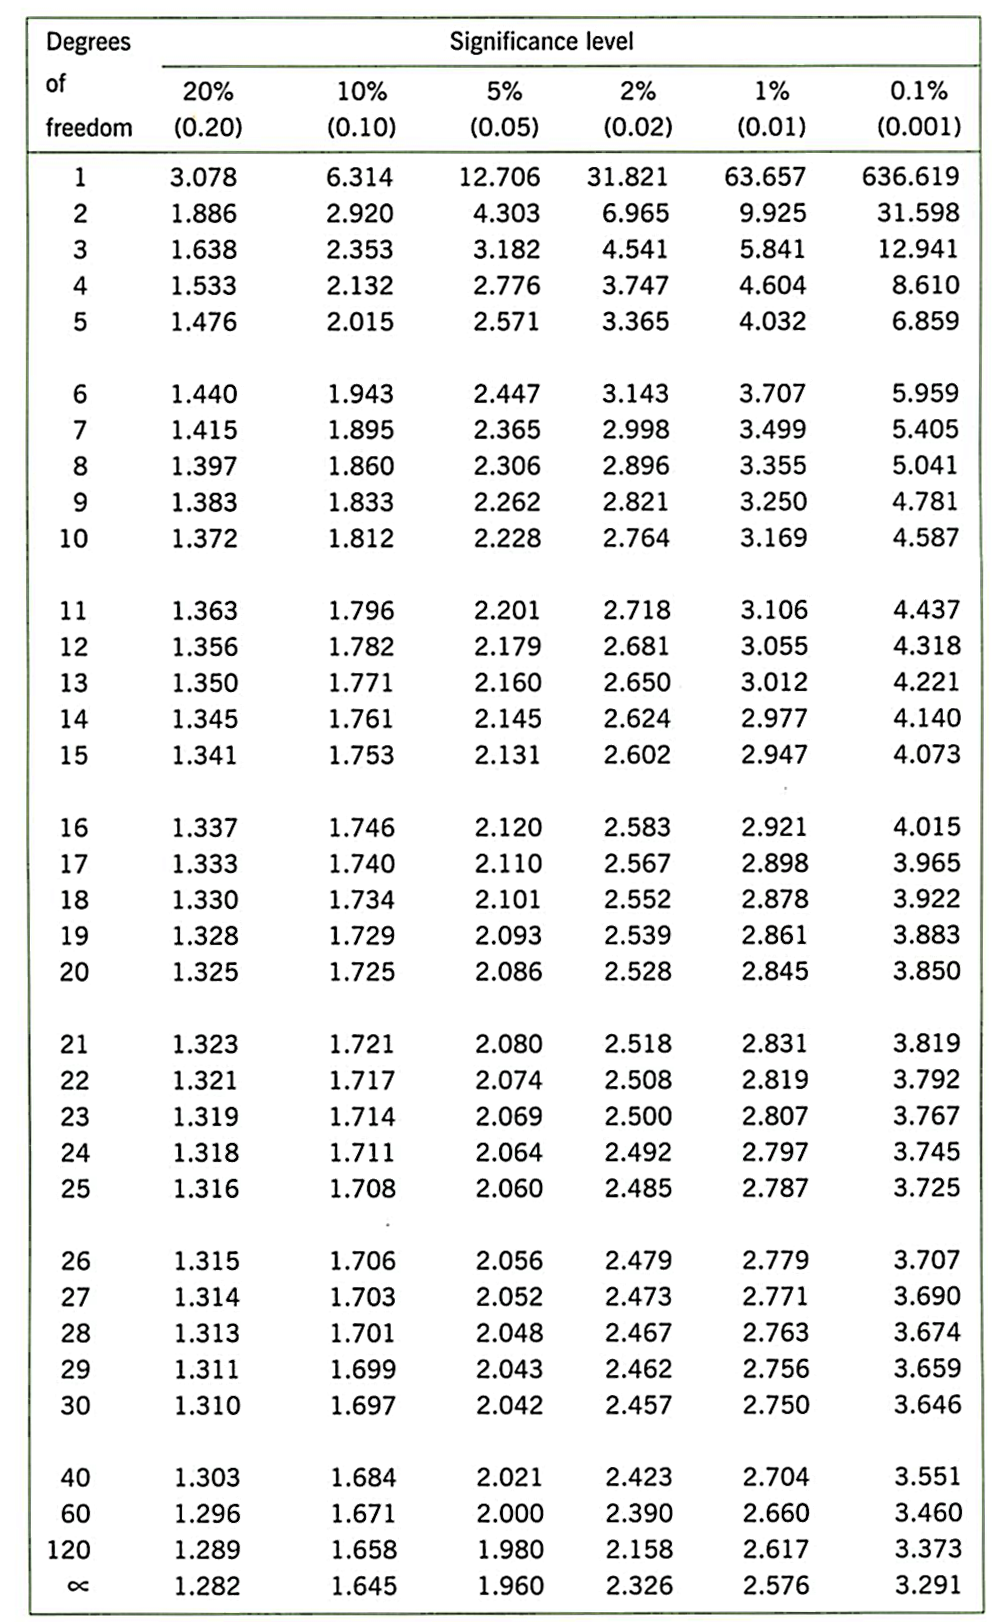
\includegraphics{files/Week_7/ttable.png}

\hypertarget{plotting-salary-estimates-by-home-location}{%
\subsection{Plotting salary estimates by home location}\label{plotting-salary-estimates-by-home-location}}

\begin{enumerate}
\def\labelenumi{\arabic{enumi}.}
\setcounter{enumi}{8}
\item
  Draw density plot
\item
  Map the fill aesthetic to the variable \emph{home\_location}
\item
  Manually change the colours of the columns by adding (+) this code as a layer to your ggplot code: \texttt{scale\_fill\_manual(values\ =\ c("darkgreen",\ "darkblue",\ "darkred"))}. Click here {[}add link{]} for a guide to colours - more than you'll probably ever want!
\item
  Click Export-\textgreater Save as Image.
\end{enumerate}

\hypertarget{week-7-plotting-means-and-ses}{%
\chapter{Week 7: Plotting means and SEs}\label{week-7-plotting-means-and-ses}}

\begin{quote}
Written by Tom Beesley \& John Towse
\end{quote}

Today we will continue to develop our skills in \textbf{data visualisation} with the \texttt{ggplot()} commands. We will look at plotting means and standard errors, and at how geoms can share aesthetic mappings. We will explore our data on the famous ``Stroop Task'' and calculate

\hypertarget{pre-lab-work-online-tutorial-2}{%
\section{Pre-lab work: online tutorial}\label{pre-lab-work-online-tutorial-2}}

\textbf{Online tutorial}: To access the \href{https://ma-rconnect.lancs.ac.uk/Week_7_LabPrep}{\textbf{pre-lab tutorial click here}} (on campus, or VPN required)

\textbf{Getting ready for the lab class}

\begin{enumerate}
\def\labelenumi{\arabic{enumi}.}
\item
  Create a folder and a Project for Week 7. \protect\hyperlink{creating_project}{Click here for the instructions} from last week if you are unsure.
\item
  Download the \href{files/Week_7/Week_7.zip}{Week\_7.zip} and upload it into this new folder in RStudio Server. If you need them, \protect\hyperlink{uploading_zip}{here are the instructions} from Week 2.
\end{enumerate}

\hypertarget{rstudio-task-1}{%
\section{RStudio Task 1:}\label{rstudio-task-1}}

The ``Stroop Effect'' is a classic demonstration of automaticity of behaviour. Participants have to say the colour a word is printed in, which is an easy task for a ``compatible'' stimulus like \textcolor{green}{GREEN}, and a much more difficult task for an ``incompatible'' stimulus like \textcolor{red}{BLUE}. We can't help but read the text - it has seemingly become an automatic process.

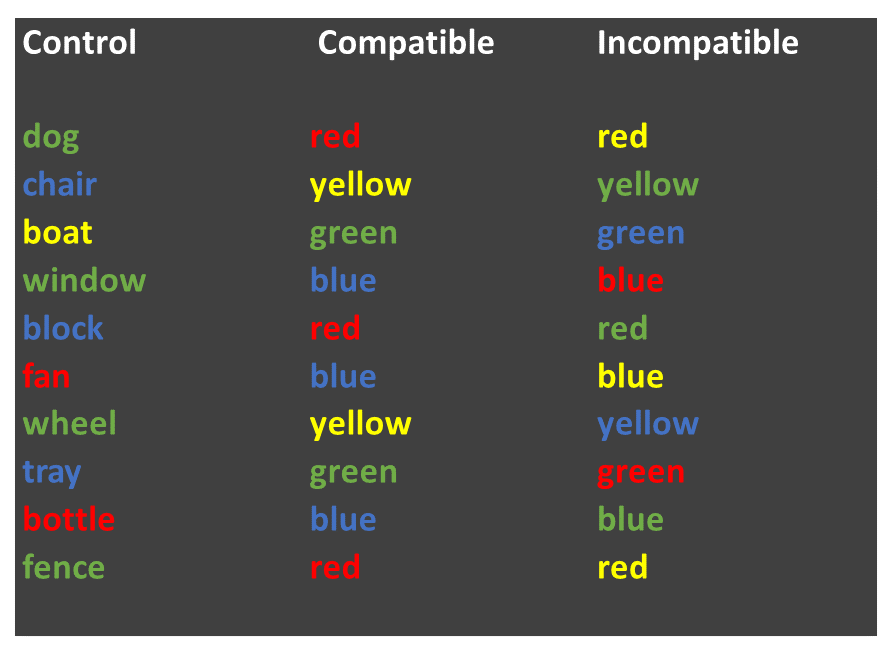
\includegraphics{files/Week_7/stroop.png}

In this task we will calculate the means and standard errors of the means. We will then plot them using ggplot().

\begin{enumerate}
\def\labelenumi{\arabic{enumi}.}
\item
  Open the script ``Week\_7\_Tasks.R'' (if you've missed them, see the pre-lab steps above). \textbf{Important!} Use this script to complete the task. You should edit this as you go through the tasks, add comments to the code (\#) and save this as a record of your completed lab work
\item
  Run the first two lines of code \texttt{library(tidyverse)} and \texttt{data\ \textless{}-\ read\_csv("data\_stroop.csv")}
\item
  View the data with \texttt{view(data)}. You will see that the data are a little different from the data we have worked with previously. We have an ID variable, which gives a unique number for each person. Each person has 3 rows. This is because the different conditions of the stroop task is a \emph{within-subjects} variable. For data like this it is often useful to have them arranged in what is referred to as ``long format'', with multiple rows for each response the participant provided. For the current data that means we have a variable called \emph{stroop\_condition}, which is our IV, and one called \emph{stroop\_time} which is our DV.
\item
  Return to the Week\_8\_Tasks.R script. You will see we have provided you with the ``scaffold'' of a complete analysis process for the Stroop data. The raw data will be grouped and then summarised as means and SEs, and then plotted with columns and error bars. This is very similar to the commands used at the end of the learnr tutorial, and you can refer to that analysis if you get stuck here. \textbf{Your job is to carefully work through the code and fill in the parts that are marked MISSING}. By the end, you should have a graph with 3 columns, with the standard error of the means plotted on top.
\item
  Add a \texttt{labs()} layer to the plot to change the axis titles, and the title of the plot.
\item
  Change the theme of the plot
\item
  Map the fill aesthetic to the variable \emph{stroop\_condition}
\item
  Manually change the colours of the columns with (e.g.) \texttt{scale\_fill\_manual(values\ =\ c("darkgreen",\ "darkblue",\ "darkred"))}. Open the RColor.pdf in the Week 8 files for more colours than you'll probably ever want!
\item
  Click Export-\textgreater Save as Image. Then show it off to the world (i.e., the Teams channel)
\end{enumerate}

\end{document}
